\documentclass{article}
\usepackage{caption}
\usepackage[
  paperheight=8.5in,
  paperwidth=5.5in,
  left=10mm,
  right=10mm,
  top=20mm,
  bottom=20mm]{geometry}
\usepackage[utf8]{inputenc}

\usepackage{graphicx}
\usepackage{wrapfig}
\usepackage[bottom]{footmisc}
\usepackage{listings}
\usepackage{enumitem}

\usepackage{wrapfig}
\usepackage{ragged2e}

\usepackage{array}
\usepackage[table]{xcolor}
\usepackage{multirow}
\usepackage{booktabs}
\usepackage{hhline}
\definecolor{palegreen}{rgb}{0.6,0.98,0.6}

\usepackage{amsmath}
\usepackage{amssymb}
\usepackage{multicol}
\usepackage{lipsum}
\usepackage{hyphenat}
\PassOptionsToPackage{hyphens}{url}
\usepackage{url}

\usepackage{rotating}

%\usepackage{xeCJK}

%% support use of straight quotes in code listings
\usepackage[T1]{fontenc}
\usepackage{textcomp}
\usepackage{listings}
\lstset{upquote=true}

%% for shrinking space between lines
\usepackage{setspace}

\newcommand*{\affaddr}[1]{#1} % No op here. Customize it for different styles.
\newcommand*{\affmark}[1][*]{\textsuperscript{#1}}
\newcommand*{\email}[1]{\small{\texttt{#1}}}
\newcommand{\tarot}{\textsc{Tarot}}
\renewcommand*\contentsname{\centering Table of Contents}

\renewcommand{\footnoterule}{%
  \kern -3pt
  \hrule width \textwidth height 0.5pt
  \kern 2pt
}

% remove date
\date{}

\usepackage{titlesec}
\titleformat*{\section}{\large\bfseries}
\titleformat*{\subsection}{\normalsize\bfseries}
\titleformat*{\subsubsection}{\normalsize\bfseries}

\usepackage{biblatex}


\usepackage{algorithm}
\usepackage{algpseudocode}

\addbibresource{sample.bib}

\title{Investigation of Social Cognitive Factors Affecting Computing Transfer Students
\footnote{\protectCopyright \copyright 2024 by the Consortium for Computing Sciences in Colleges.
Permission to copy without fee all or part of this material is granted provided
that the copies are not made or distributed for direct commercial advantage,
the CCSC copyright notice and the title of the publication and its date appear,
and notice is given that copying is by permission of the Consortium for
Computing Sciences in Colleges.  To copy otherwise, or to republish, requires
a fee and/or specific permission.
}
}
%Original title----Exploratory Analysis of Social and Personal Factors Impacting Student Success
%Author list for 8 below.
\author{
Kay Vargas\affmark[1],  Victor Diaz\affmark[1],  Claire MacDonald \affmark[3]\\
 Yun Wan\affmark[4], Xiwei Wang\affmark[5], Palvi Aggarwal\affmark[3]\\
 Shebuti Rayana \affmark[2] and Sherrene Bogle \affmark[1]\\
\affmark[1] California State Polytechnic University Humboldt, Arcata, CA\\
\email{\{kv111, vmd21, sab30\}@humboldt.edu}\\
\affmark[2]SUNY OLD Westbury, Albany, NY\\
\email{rayanas@oldwestbury.edu}\\
\affmark[3]University of Texas At El Paso, TX\\
\email{cemacdonald2@miners.utep.edu}, \email{paggarwal@utep.edu}\\
\affmark[4]University of Houston-Victoria, Victoria, TX\\
\email{wany@uhv.edu}\\
\affmark[5]Northeastern Illinois University, Chicago, IL\\
\email{xwang9@neiu.edu}

}
%\author{
%Baochuan Lu\affmark[1] and John Meinke\affmark[2]\\
%\affmark[1]Computer and Information Sciences\\
%Southwest Baptist University\\
%Bolivar, MO 65613\\
%\email{blu@sbuniv.edu}\\
%\affmark[2]Computer Science Department\\
%Another University\\
%Our Town, TX 00000\\
%\email{jmeinke@univ.edu}\\
%}

\begin{document}
\maketitle
\thispagestyle{empty}
\pagestyle{empty}

\begin{abstract}
 %Of the students enrolled in community colleges, 29\% are first generation, along with 42\%  black and 52\%  Hispanic students. 
 There is a disproportionate racial and ethnic enrollment of students in community colleges. %Among the students currently enrolled in community colleges, 29\% identify as first-generation, while 42\% are Black, and 52\% are Hispanic.
 Alongside this disproportionate enrollment, underrepresented minority (URM) students also have lower retention rates than their peers. While the literature addresses some of the factors that impact students' degree completion, there still exists a gap in overarching factors that affect URM students. This study aims to explore the specific personal and social factors that impact URM Computing transfer student success. Specifically, exploring factors using Bandura's social cognitive theory (SCT). %~\cite{bandura1986social}.
Data was gathered with two methods, one-on-one interviews with students and a self-assessment of the student's abilities in the three categories of the SCT: self-efficacy (SE), outcome expectation (OE), and goal setting (GS). The analysis showed that the average rating of the SE and GS of post-transfer students was slightly higher than the Pre-transfer group. Moreover, stratification of word clouds from surveys of the data showed overarching factors between pre and post-transfer groups. Pre-transfer students were impacted by time and income. 
\end{abstract}

\section{Research Problem}
In recent years the need for a large workforce specializing in STEM fields has increased. However, along with the need for more workers there has also been a focus on decreasing disparities in the representation of diverse populations in STEM. The U.S. Census Bureau lists 71\% of STEM workers as non-Hispanic white with only 6\% and 7\% being black or Hispanic, respectively. Similarly, only 13\% and 27\% of engineers and computer scientists are women~\cite{landivar2013disparities}. Part of this disparity can be attributed to the lack of representation and persistence of underrepresented minority (URM) students in colleges. To begin addressing these disparities in the workforce it is imperative to build an understanding of the factors impacting URM success in college specifically at the community college (CC) level as many URM students begin their journey there. Among the students enrolled in community colleges 29\% are first-generation along with 42\% and 52\% of all Black and Hispanic students beginning their academic journey at CC~\cite{chamely2021undergraduate}. 
As~\cite{chen2015community} states, “For many ... URM populations, community colleges serve as an entry point to post secondary education and offer a unique opportunity in the preparation of a future STEM workforce that reflects the diversity of the U.S. population”.
In order to build a more diverse workforce that is representative of the population, URM students must be properly supported and have the needed resources to be successful at CC and 4-year institutions.
While the literature extensively covers academic factors affecting URM transfer success, in order to establish more equitable practices and support, a holistic understanding of the social and behavioral factors of URM students is crucial.
%While academic factors impacting URM transfer success have been well documented in the literature, there is a need to understand the role social and behavioral factors play in student success. %While behavior encompasses a large range of actions with complex underpinnings, understanding the underlying self-perspectives which drive and are predictive of action may offer much insight into URM transfer success and behaviors.%
%In having a more holistic understanding of URM students there is a larger capacity to create more equitable practices and support for these students.
The authors have previously examined personal and academic factors impacting transfer students ~\cite{BlindAuthors2023}, so this paper focuses on social and behavioral factors, specifically aspects of Bandura’s Social Cognitive Theory~\cite{bandura1986social}.
%(\textbf{10}) single-spaced pages including tables, figures, and a list of references or bibliography.

\section{ Review of Related Literature}
\subsection{Behavioral factors}
\small
%Schlossberg's transition theory \cite{schlossberg1989marginality} states that any transition will change the relationships, routines, assumptions, and roles of an individual. An important step in the transition process is the individual's perception. They will decide whether the change qualifies as a transition or not. According to Schlossberg's theory, attending university is a transition, which means that how students cope with university will be influenced by the Situation, their Self, Support, and Coping Strategies. %Schlossberg's transition theory also outlines four personal factors that determine an individual's ability to cope with a transition: situation, self, support, and strategies. The Situation factor pertains to the elements of the transition, such as how it is occurring, its duration, its level of stress, and whether the individual can change the situation. %
%The Self factor has two categories: personal/demographic and psychological resourcefulness. Social support includes all of an individual's relationships and how they provide support. The last major factor is Coping Responses, which are categorized into three strategies: changing the situation, controlling the meaning of the problem, and managing the stress of the situation. Transfer students who have been exposed to an academic environment before tend to cope better with university based on this theory. Schlossberg's theory identifies the other three major factors that affect students, which are self, support, and coping strategies.
%This study will focus on the social and behavioral factors that impact transfer student success.%

%As of 2020, 40\% of all 18-24-year-olds were enrolled in a postsecondary program ~\cite{welding2023}.  Research has shown that ``relatively good graduation rates for community college transfers get even better for students who complete their associate degree before heading to a four-year institution'' \cite{fain2012} %Jaschik
%and that ``in the UC (University of California) system, transfer student graduation rates are better than their freshman graduation rates'' \cite{uc2021}. Understanding the factors that drive student success is a key element in education. %Schlossberg's theory identifies the other three major factors that affect students as Self, Support, and Coping Strategies.
%This study will focus on the social and behavioral factors that impact transfer student success.

%\textbf{Figure goes here}
%\includegraphics[scale=0.75]{image/Figure_1.png}
Previous research has identified elements such as engagement with communities, social belonging, academic uncertainty, and the transfer process, which impact the success of transfer students. Transfer students have a higher success rate when engaging with the community \cite{ucregents2022}. There is additional success when students feel that they have course-level social belonging \cite{edwards2021relationship}. A decline in academics stems from situations where students try to balance work with academics and relationships or do not have a sense of belonging, leading to a feeling of academic uncertainty \cite{hohne2019belonging}. Transfer students have less time in the new environment, so it is harder for them to adapt \cite{blekic2020continuing}


%Previous research has seen elements such as engagement with community, social belonging, academic uncertainty, and the transfer process impacting the success of transfer students. Engaging with the community helps transfer students succeed \cite{ucregents2022}.
%Academic uncertainty causes students to think of their profession rather than their major, making them think of other pathways, rather than school \cite{reid2021reaching}. Having academic uncertainty can be a predicting factor in a student's dropout intentions \cite{hohne2019belonging,lederman2020progress}.
%Students who try to balance work along with academics and relationships have more of a challenge when trying to achieve a balance. In these cases, it can cause a decline in academics.  Students who feel that they have course-level social belonging tend to do better in their courses \cite{edwards2021relationship}  than those who do not have a sense of belonging who often charter a feeling of academic uncertainty \cite{hohne2019belonging}. Transfer students have less time in the new environment, so it is harder on them to adapt \cite{blekic2020continuing}
%Getting credit approval in the transfer process from one’s institution creates added stress which makes it harder for students to succeed \cite{lederman2020progress}. Lack of credit transfer makes students retake classes causing them to stay in school for a longer period \cite{lederman2020progress}. Transfer students have less time in the new environment, so it is harder on them to adapt \cite{blekic2020continuing}. %Wang [7] shows social inhibitions as another factor whereby when socializing becomes harder, or a challenge, students will not participate.

\subsection{Conceptual Framework}
\enlargethispage{\baselineskip}

\small
%\includegraphics[scale=0.6, center]{image/Figure_1.png}

Bandura’s Social Cognitive Theory (SCT)~\cite{bandura1986social}, depicted in Figure \ref{fig:bandura} was used as a working guide for understanding the underlying personality traits driving student success. The SCT serves as a psychological framework used to understand the relationship between environmental factors and one's motivation, learning, and self-regulation \cite{schunk2019}. 
Under this model, it is understood that an individual's self-conception and personal beliefs will be a greater predictor of their future success rather than their previous achievements. Within this context, our interest was in evaluating students' perception of themselves quantitatively within the three constructs of the SCT, self-efficacy (SE), goal setting (GS), and outcome expectation (OE).

%\vspace{-5pt}

\begin{figure}[h]
    \centering
    \includegraphics[width=0.5\textwidth]{Figure_1.png}
    \captionsetup{font=scriptsize} % Set the font size for both caption and label
    \caption{Model of the relations between the three classes of determinants in Bandura's (1986) conception of triadic reciprocity}
    \label{fig:bandura}
\end{figure}
\vspace{-5pt}




%\subsubsection{Self-Efficacy and Academic Performance}
\small
\textbf{Self-efficacy} can be defined as an individual's belief in their own capacity to be successful in achieving a given goal. SE is identified as a factor in predicting student behavior and overall academic performance \cite{kozlowski2020measuring}. As stated by \cite{pajares1996self}, “Efficacy beliefs help determine how much effort people will expend on an activity%, how long they will persevere when confronting obstacles, and how resilient they will prove in the face of adverse situations %
-- the higher the sense of efficacy, the greater the effort, persistence, and resilience (p544).” Self-efficacy is thought to be pivotal to the human agency as a person will not participate in an activity if they do not believe that they can produce results \cite{kozlowski2020measuring}. \cite{bogle2018undergraduate} used the SCT model and SE was found to be the most dominant predictor of academic performance among a sample of 404 high school Information Technology students.

%\subsubsection{Goal Setting and Academic Performance}
\small
\textbf{Goal-setting} is the behavior of setting a goal for the future and actively taking steps to eventually achieve it. Bandura~\cite{bandura1986social} indicates learners are motivated by goals and plan and execute their behavior accordingly.

%\subsubsection{Outcome Expectation and Academic Performance}
\small
\textbf{Outcome expectation} is the anticipated result of engaging in a given behavior. OE is not thought to be as significant as self-efficacy in predicting a student's performance, rather it is thought that there is an interplay between the two constructs in an individual's overall behavior. As stated by Bandura, “In social, intellectual, and physical pursuits, those who judge themselves highly efficacious will expect favorable outcomes…”~\cite{bandura1986social}.

%\textbf{Figrue goes here}
%\includegraphics[scale=0.75]{image/Figure_1.png}{\label{fig:q3b}}

\section{Methodology}
\small
This study used data derived from the self-report Likert scale, interviews, and survey responses. This form of measurement allows for collecting quantitative data for otherwise unmeasurable constructs. Since understanding a student's self-perception under the SCT model was not otherwise directly accessible, this data collection method allowed insight into the needed modalities. Furthermore, the data was then analyzed with two methods under the three previously defined constructs within the SCT and by stratification with word clouds.

\subsection{Integration of Framework}
\small
The population consisted of students attending both community colleges (CC) and 4-year institutions in four different states.  All students were enrolled in a computer science or related program, and students had either transferred to a 4-year institution after attending CC or were currently enrolled in a CC. The interviewees' data was evaluated under the SCT, and the dependent variables used were GS, OE, and SE, while the independent variable was transfer status. The transfer student data set was analyzed using first-generation status, low-income status, ethnic minority, and sex as independent variables. The dependent variables were average transfer GPA, average overall GPA, and average increase from transfer GPA to institutional GPA.


% \subsection{Target Population}
% \small
% Our population consisted of students attending both CC and 4-year institutions in four different states.  All students were enrolled in a computer science or related field and students had either transferred to a 4-year institution after attending CC or were currently enrolled in a CC.

\subsection{Data Collection Method}
\small
The SCT data was collected by interviews with 15 students from the target population and a self-reported survey of 65 students. The interview consisted of several questions aimed at assessing students' decision-making processes: SE, OE, and GS.  These interviews were comprised of six or seven questions depending on whether students were currently attending CC with an intent to transfer (six questions) or had already transferred to a 4-year institution (seven questions).
Consequently, the data from particular questions in both interviews and surveys were utilized to create word clouds, examining issues relevant to both pre-transfer and post-transfer students. 

The first five questions were open-ended questions that allowed students to describe their personal and academic experiences. Questions 6 and 7 were closed-ended questions with self-reported measurements of their own personal OE, GS, and SE. This was measured by asking students to rate themselves in terms of their self-perception as a highly confident student, as someone who sets goals each semester, and as one who is motivated by previous experiences of self and others.
%This question utilized a five-point Likert scale as follows: 
For the stratification within the survey segment, a word cloud was created, and the questions where the word cloud was utilized included a pre-transfer question (Q16) that asked the respondents to list the information they used when deciding between a community college and a 4-year university. Additionally, they were prompted to mention any information they felt was needed but not available, such as the proximity of a 4-year university, better job opportunities at a 4-year university, ease of transfer, cost considerations, and guidance from family and friends. For the post-transfer word cloud stratification, a combination of interview and survey questions was employed. The relevant post-transfer questions (Q6 and 25) requested participants to share  any particular experiences they deemed important as a transfer computing major student.





%\textit{Question 6} – On a Likert scale of 1-5 where 1 represents lowest and 5 represents highest, how do you rate yourself on the following: a) self-efficacy, b) goal setting, and c) outcome %expectation? The question rated pre-transfer rankings at the CC. Students at the four-year institution were asked to rank their SCT factors after transfer in Question 7.
%Word cloud analysis was performed on a survey of 65 students across five states.

 \section{Results}
Evaluating under the SCT model, the hypothesis was that students who had already transferred from CC to a 4-year university would on average rate themselves higher in SE, GS, and OE. The expectation is that students who successfully transferred would have a higher self-rating specifically in SE as indicated by their previous success \cite{chen2014influence, dutta2015social, jung2017self, luo2021stem,pajares1996self}.
%[23]
As seen in Figure 2, %\ref{fig:q67}% 
it was found that the average rating of the group of post-transfer students was slightly higher than the pre-transfer group in both measurements of SE and GS. However, it should be noted that the sample size for the two groups was not even and a larger sample size would allow for a more accurate reflection. Similarly, the students interviewed in the pre-transfer group consisted of individuals who intend to transfer to a 4-year institution. For this reason, it is possible that this group already had higher levels of self-perception in the given constructs as they already held this expectation for themselves. In the future having a sample population of students who do not intend to transfer out of CC to a 4-year institution would allow for better insight into the correlation of these constructs on student persistence to transfer. 
%\includegraphics[scale=0.42]{image/Figure_8.png}

\vspace{-5pt}
\begin{figure}[h]
\centering
\begin{tabular}{cc}
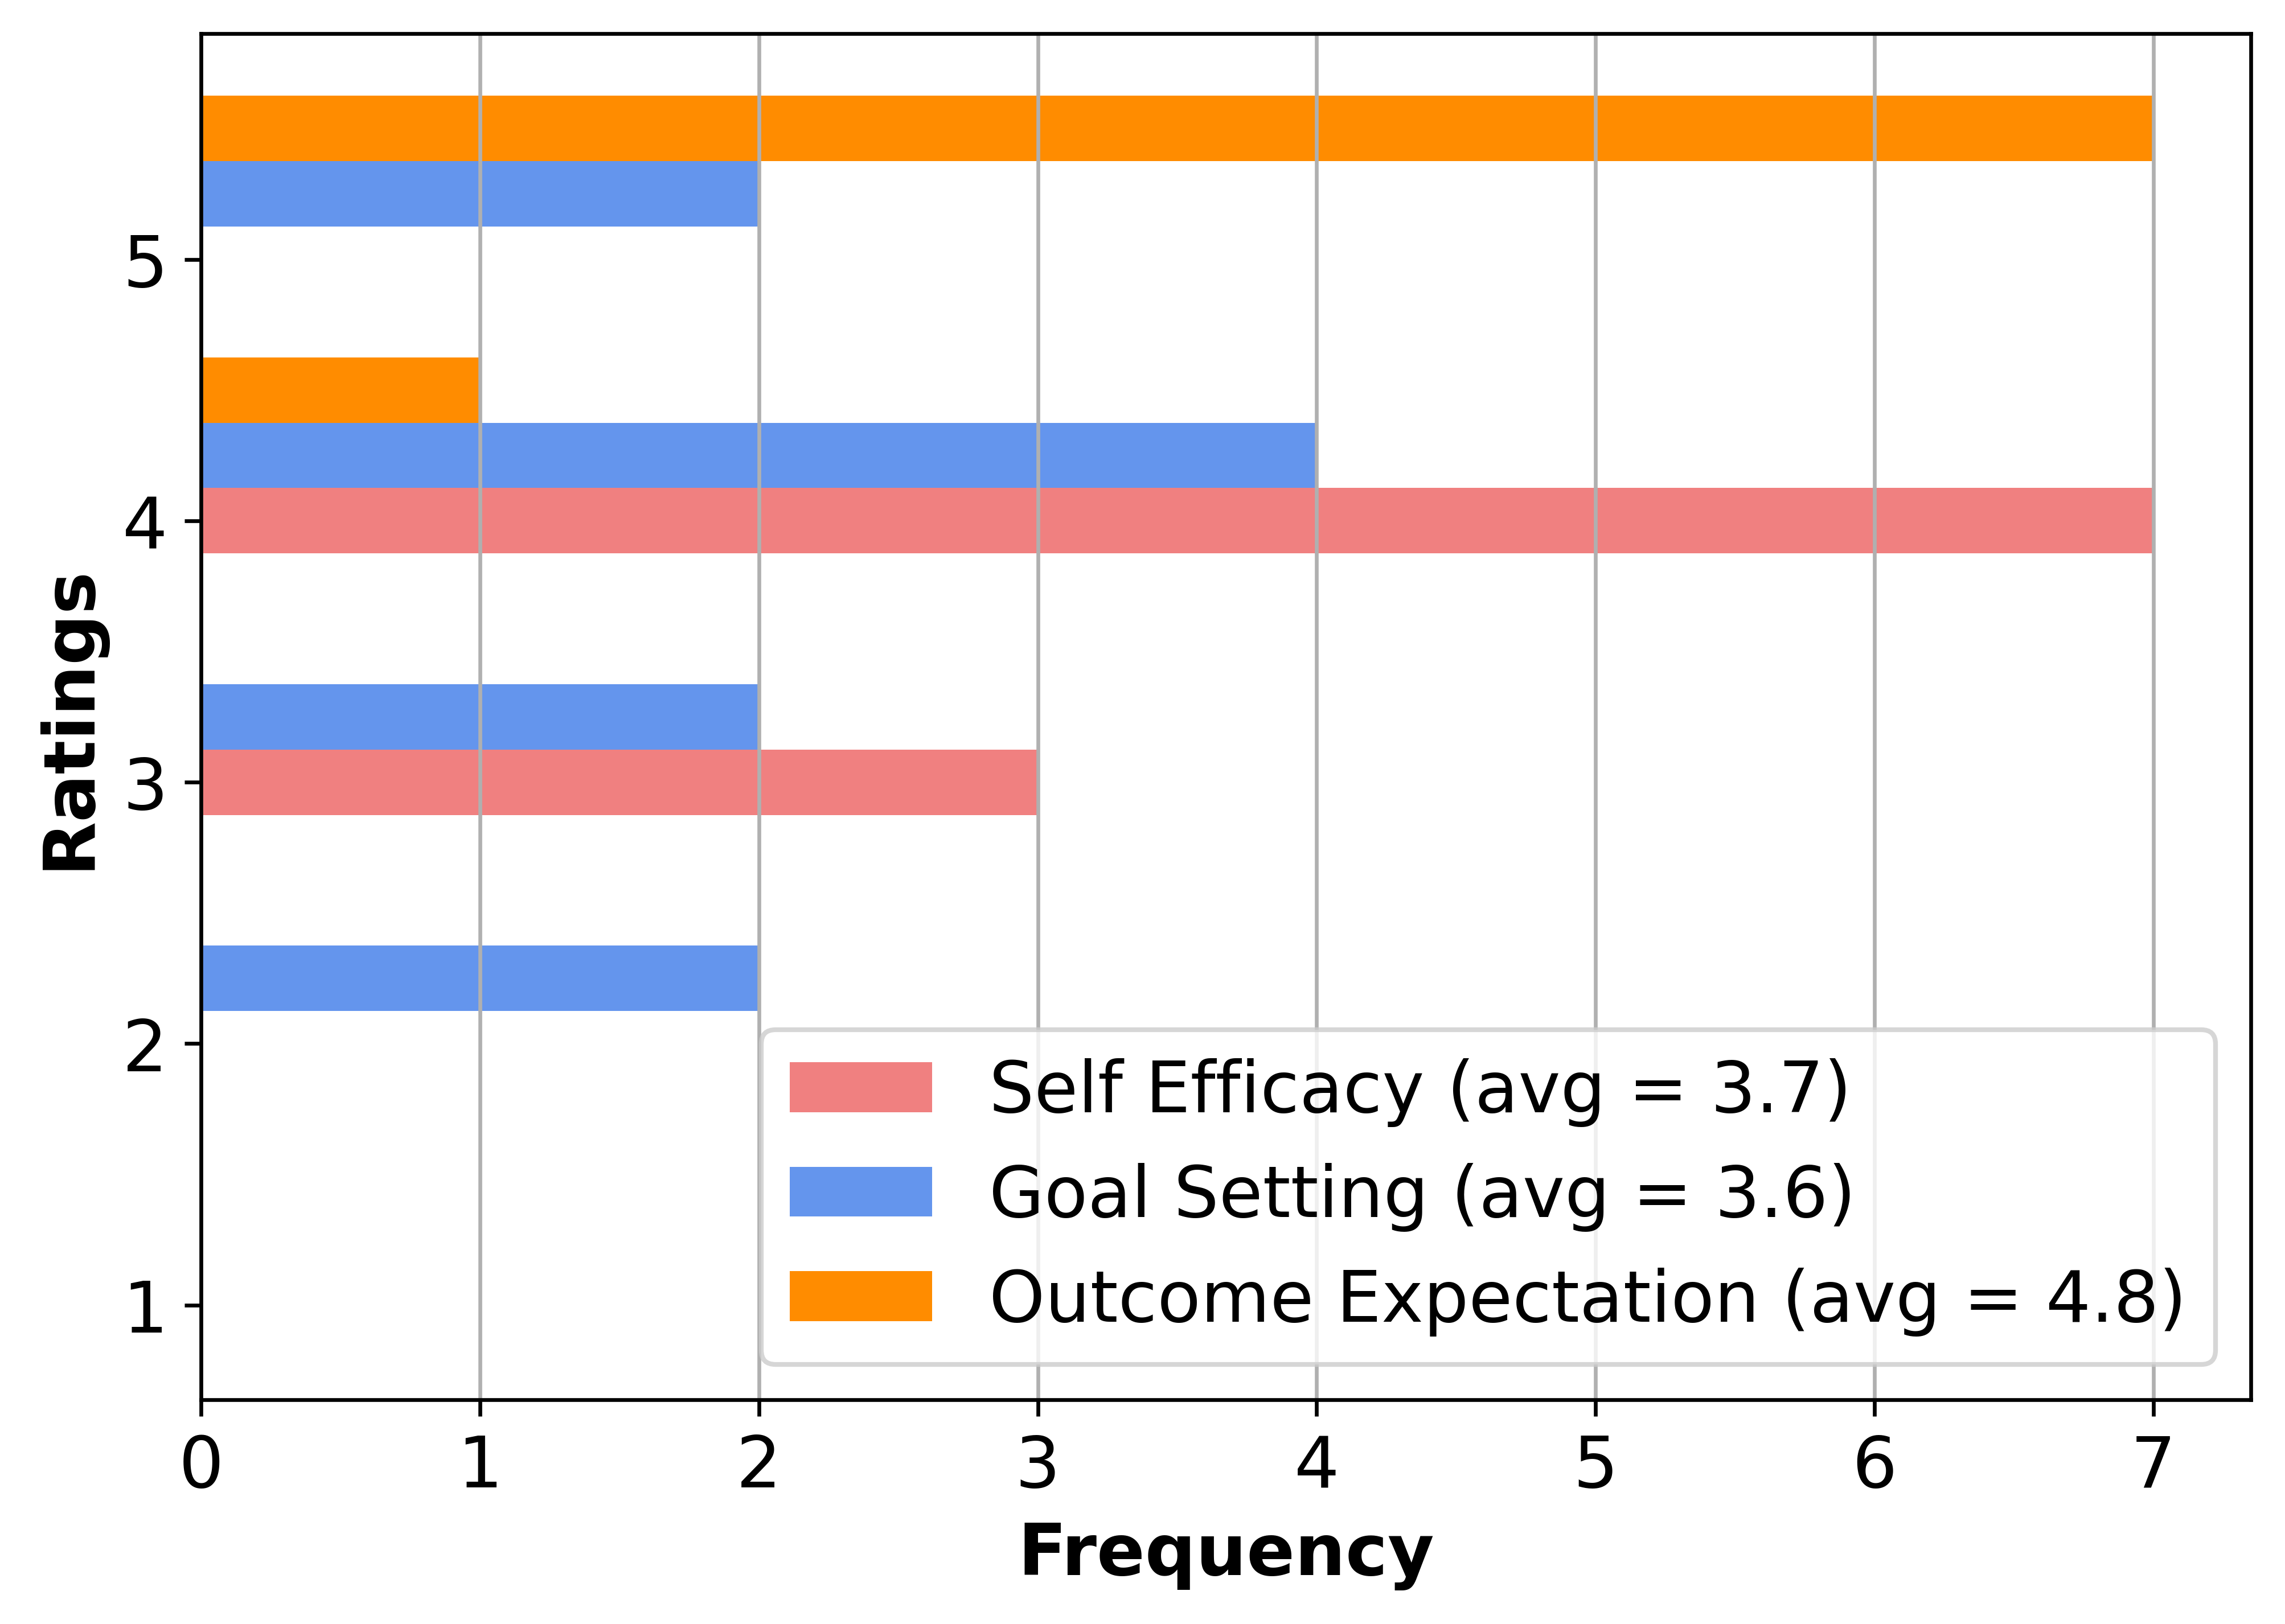
\includegraphics[width=0.49\textwidth]{Q6.png} & 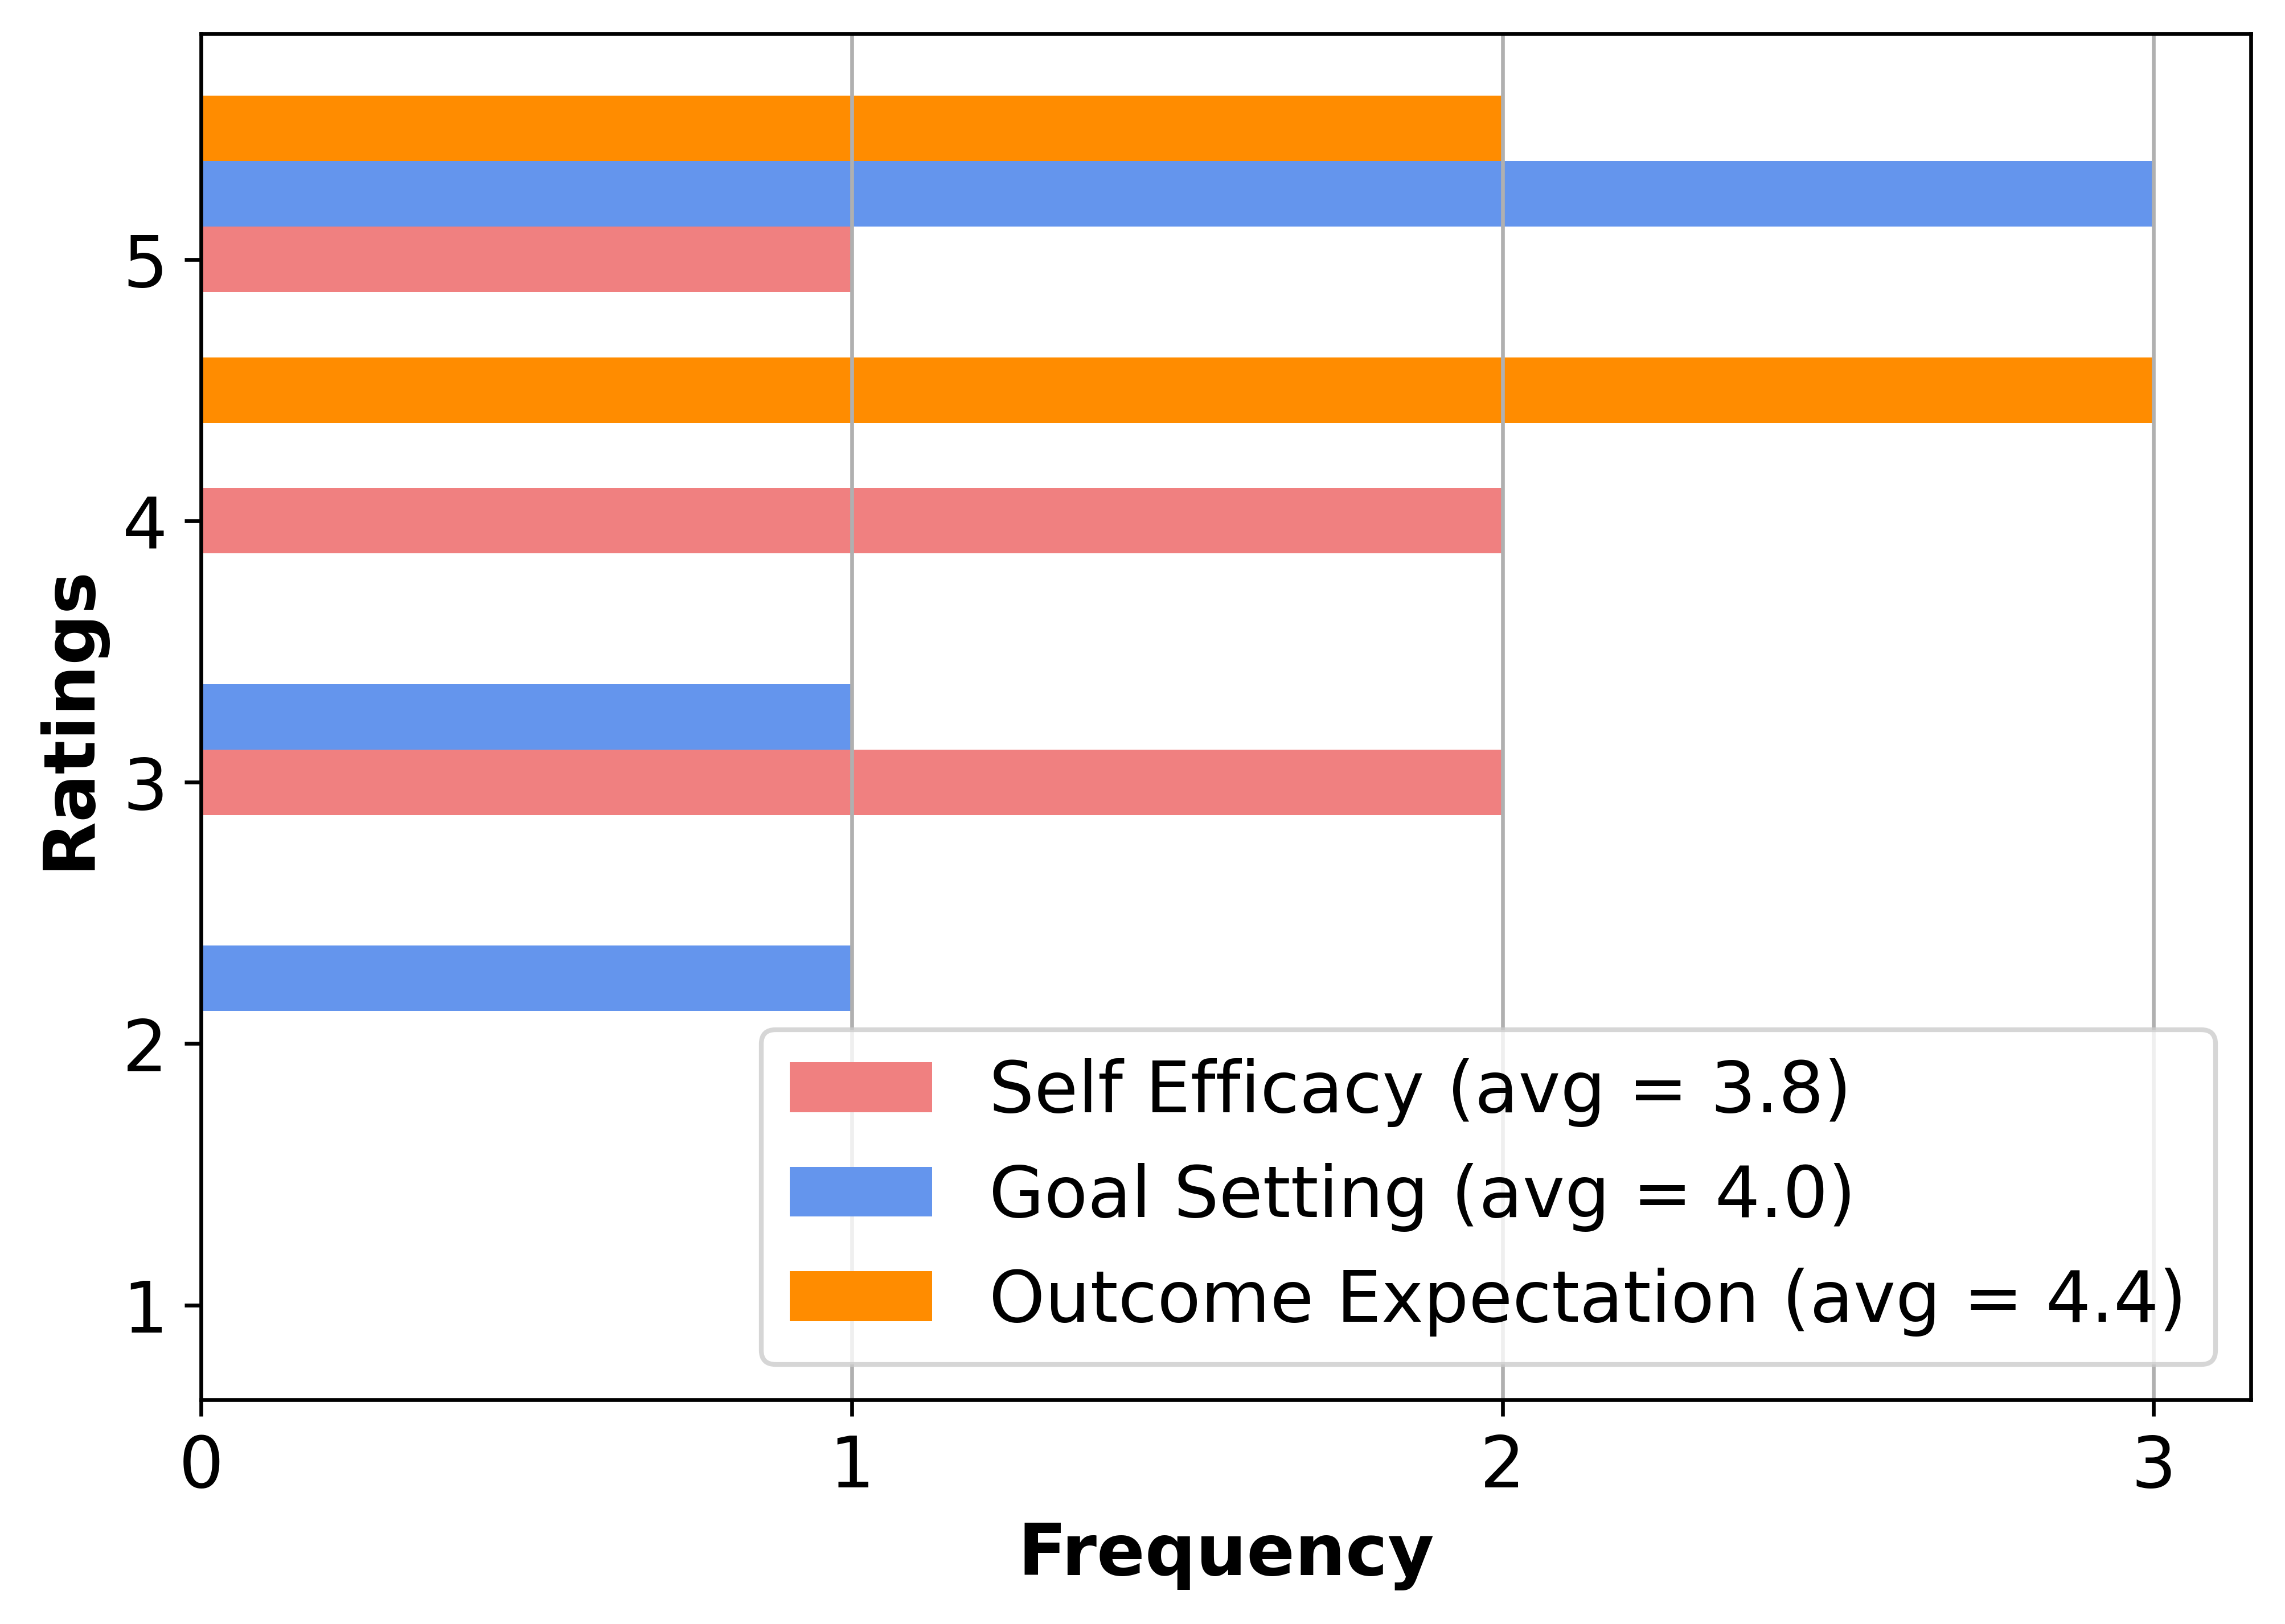
\includegraphics[width=0.49\textwidth]{Q7.png} \\
   {\footnotesize (a) Pre-Transfer} & {\footnotesize (b) Post-Transfer}\\ 
    \end{tabular}
    \vspace{-5pt}
     \caption{Student responses to Questions 6 (a) and 7 (b)}
    \label{fig:q3a}
\end{figure}

\begin{figure}[h]
\centering
\begin{tabular}{cc}
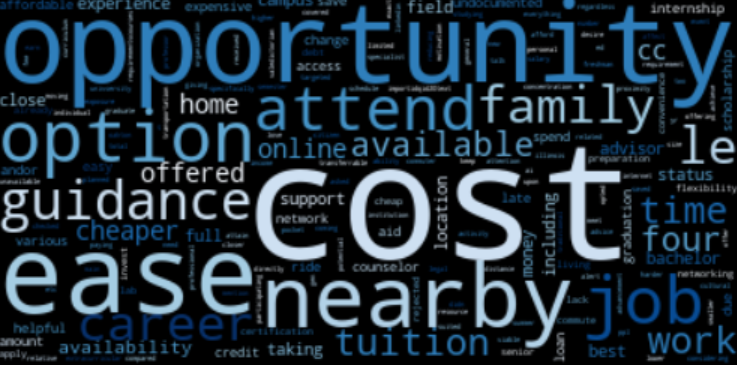
\includegraphics[width=0.48\textwidth]{Survey_Q16.png} & 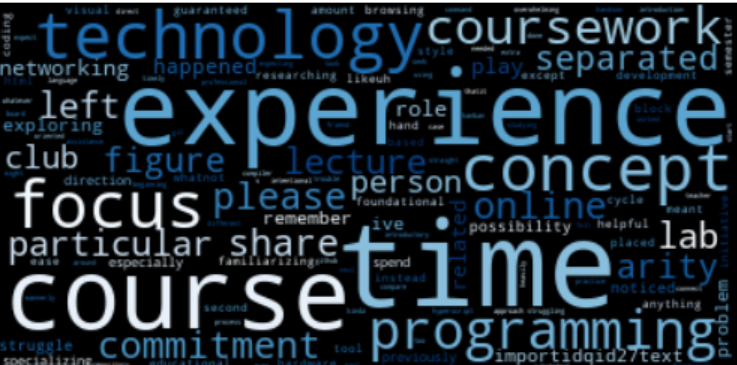
\includegraphics[width=0.48\textwidth]{Survey_Inter_Q6_25.png} \\

%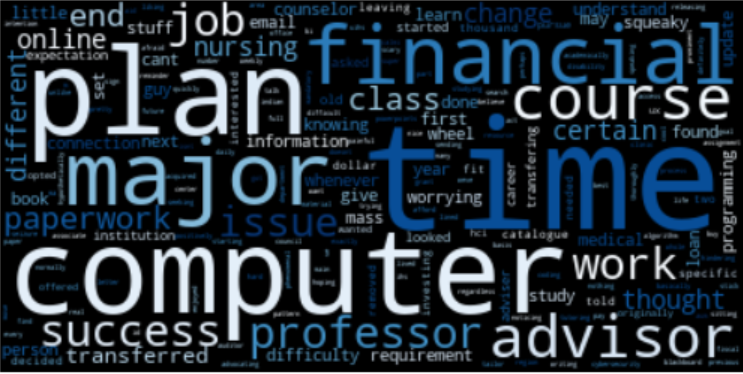
\includegraphics[width=0.46\textwidth]{Question_3_word_cloud.png} & 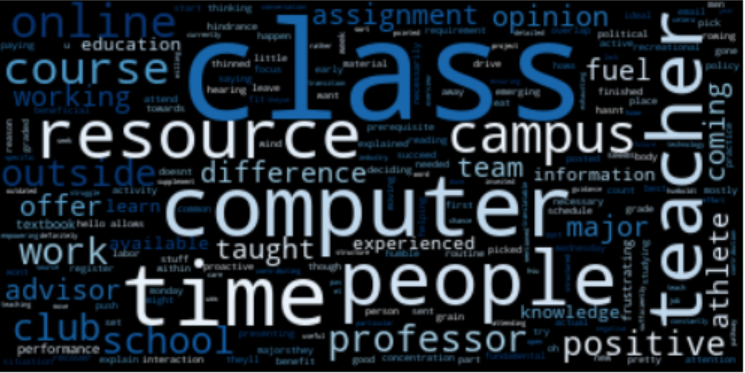
\includegraphics[width=0.46\textwidth]{Question_4_word_cloud.png} \\
   {\footnotesize (a)Pre-Transfer Survey Q16} & {\footnotesize (b) Post-Transfer Survey Q6 and Interview Q25}\\ 
    \end{tabular}
    \vspace{-5pt}
     \caption{Word clouds of  65 students’ responses}
\label{fig:q3b}
\end{figure}

% Evaluating under the SCT model, the hypothesis was that students who had already transferred from CC to a 4-year university would on average rate themselves higher in SE, GS, and OE. The expectation is that students who successfully transferred would have a higher self-rating specifically in SE as indicated by their previous success \cite{chen2014influence, dutta2015social, jung2017self, luo2021stem,pajares1996self}.
%[23]
%Figure \ref{fig:q3b} shows word clouds from students' interview responses and surveys on questions Pre-TRANSFER Question 16. In this question, respondents were asked to list the information they used when deciding between a community college and a 4-year university. Additionally, they were prompted to mention any information they felt was needed but not available, such as the proximity of a 4-year university, better job opportunities at a 4-year university, ease of transfer, cost considerations, and guidance from family and friends.
%For the Post-Transfer Word Cloud stratification, a combination of INTERVIEW/SURVEY questions was employed. The relevant questions were POST-TRANSFER Q6 and Q25. In Q6, participants were asked if there was any particular experience they deemed important as a transfer computing major student. Q25 invited respondents to share any specific experiences they felt were significant in their roles as transfer computing major students.

The most urgent concerns impacting students before transferring are time and income. Income is crucial regarding the affordability of attending a 4-year university, relying on either parental income or their own. Time is a significant factor as it affects their income situation. This stems from the notion of opportunity cost, where the more time individuals spend in school, the less time they have to earn money. 

%Time is a significant factor, emphasizing the urgency associated with the transfer process. 

%\includegraphics[scale=0.42]{image/Figure_8.png}

%\vspace{-5pt}

%\paragraph{}
\medskip
\section{Conclusion}
This paper first reported a literature review to identify the key social factors, based on the SCT theory, that influence the transfer decision, particularly for students from traditionally disadvantaged groups. Secondly, an exploratory analysis was performed on these factors by interviewing 15 current students. %inviting a small group of students from community colleges and universities to a survey that includes a wide range of questions, from demographics, pre-transfer decisions to post-transfer performance, etc. 
The results revealed that their rating of SE and GS were higher after transfer than pre-transfer. 
%The data from the SCT showed that the average rating of the group of post-transfer students was slightly higher than the pre-transfer group in both measurements of SE and GS. 
This suggests that the post-transfer students felt better about their academic success than the Pre-Transfer students.
Thirdly, word cloud analysis from a survey of 65 students indicated that cost is the main factor for CC students in deciding where to start their degree. %and after transfer %Post-transfer students attributed their success in class to resources, time, people, teachers, and campus. At the same time, the pre-transfer factors are considered time and income, and the issues lie in the sense of urgency. Interviewees, in general, wanted to have a career in their fields as soon as possible. This shows a misalignment between students' concerns and self-reported beneficial factors. Hence, this study suggests further analysis of student situations and intervention methods with a larger pool of students.
%\includegraphics[scale=0.42]{image/Figure_8.png}
 Based on these results, the survey will be extended to a larger group of students across multiple states, and the combined results from factors ascertained to design an AI-driven advising system for transfer students, particularly URMs. % of those who are from underrepresented groups.%
 The researchers anticipate that this %additional factor analysis and future studies %
 will be beneficial to transfer students, their advisors, and other stakeholders of higher education.
\section{Acknowledgments}
\small
This research was supported by the National Science Foundation (NSF) CISE-MSI award CNS-2219623 and an ASEE CyBR-MSI mini-grant under NSF award CNS-2139136. 

%\section{Appendix}
%Other word clouds and survey questions can be added here.
\clearpage
\renewcommand*{\bibfont}{\fontsize{8}{8}\selectfont}
\printbibliography
\end{document}
